%Every piece of package I've acumulated over the last years
%
%
\documentclass[a4paper,12pt]{article}
\usepackage[utf8]{inputenc}
\usepackage{imakeidx}
\usepackage{graphicx}
\usepackage{float}
\usepackage{amsmath}
\usepackage[backend=bibtex,style=verbose]{biblatex}
\bibliography{bibliography}
\usepackage{csquotes}
\usepackage{tcolorbox}
\usepackage{multirow}
\usepackage{caption}
\usepackage{afterpage}
\usepackage{wrapfig}
\usepackage[margin=1in]{geometry}
%End of packages
%
%
%
\begin{document}

\title{Gyroscope}
\author{Gabriel D'Andrade Furlanetto - XDD204950}
\maketitle


\abstract{In this paper, we will analyze the motion of the gyroscope using data collected during University of Salamanca's Mechanics and Waves Laboratory class. We will pay special attention to its rotation and precession, analyze the relation between their frequencies, and then use that data to to calculate the moment of inertia of the principal axis of our system. We will then calculate the moment of inertia by using the gyroscope as a pendulum, and finally compare the two results.}
\pagebreak 
\section{Introduction}

\subsection{Objectives}

The main objective of this paper is to study the gyroscope and its movement, namely its rotation, precession and nutation. Special consideration will be given to the first two, and as such, the frequency of rotation and 

Furthermore, we will calculate the principal moment of inertia of our gyroscope in two different manners: Firstly, using the frequencies of precession and rotation; Then, using a different experimental setup that uses the gyroscope as a pendulum.

\subsection{Theoretical Introduction}

\subsubsection{The motion of the gyroscope: Rotation, precession and nutation}
To accurately describe the motion of the gyroscope, a full theory of the rigid solids is necessary. However, anyone who has come in contact with it will know that setting up the Euler Equations and solving them is an extremely non-trivial task that would be way beyond the scope of this section. We will instead consider a simplification where we consider the angular velocity to be large enough\footnote{This approximation is usually referred to as the fast (heavy) symmetrical top, and the general case is called, not surprisingly, the (heavy) symmetrical top. Solutions for the spinning top are usually covered in graduate-level Classical Mechanics texts, with our situation being used as a limiting case. If one wishes to see a detailed solution, \cite[208]{goldstein} is a great resource}. 


We will start, as is often the case in dynamics, by choosing proper coordinates for our problem. Because of the fact that the distance from the point of contact to the center of mass constant during motion, we will employ spherical polar coordinates $(r,\theta,\phi)$, as represented in Figure \ref{coord_system}. We begin by analyzing the applied torques of the system, of which gravity is the only contributor:

\begin{figure}[h!]
\centering
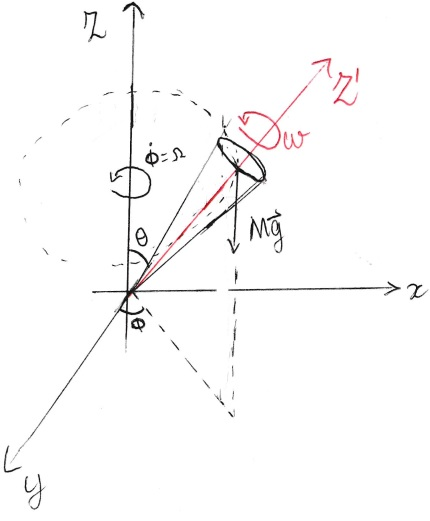
\includegraphics[width=0.25\textwidth]{coord.jpg}
\caption{Coordinate system employed in the solution of the problem}
\label{coord_system}
\end{figure} 

$\boldsymbol{\Gamma} = \boldsymbol{r} \times \boldsymbol{F} = d \boldsymbol{e_r} \times M g \boldsymbol{e_z} = M g d \boldsymbol{e_r} \times (\cos(\theta) \boldsymbol{e_r}-\sin(\theta) \boldsymbol{e_\theta})$

Where d is the distance, M is the mass of the system and g is acceleration due to gravity. If we carry out the trivial calculations, we get that 

\begin{equation}
	\label{torque}
	\boldsymbol{\Gamma} = M g d \sin(\theta) \boldsymbol{e_{\phi}}
\end{equation}

Now, we analyze the system's angular momentum. A priori, there could be a component of angular momentum in each direction, but that would give us a very complicated system to work with in the end. We will instead make use of our approximation and assume that the angular momentum along the axis of rotation, $z'$, dominates the angular momentum as a whole. As such, we write:

\begin{equation}
\label{angular}
	\boldsymbol{J} = I \omega \boldsymbol{e_r}
\end{equation}

Now, we will use the fundamental equation of the dynamics of solids:
\begin{equation}
	\label{fund}
	\frac{d \boldsymbol{J}}{dt} = \boldsymbol{\Gamma}	
\end{equation}

We know what the right side directly from equation \eqref{torque}, and we can get the left side if we take the time derivative of equation \eqref{angular}:

$$\frac{d \boldsymbol{J}}{dt} = I \left(\frac{d\omega}{dt} \boldsymbol{e_r} + \omega \frac{d\boldsymbol{e_r}}{dt}\right) = I \left(\dot{\omega} \boldsymbol{e_r} + \omega\dot{\theta} \boldsymbol{e_\theta} + \omega \dot{\phi} \sin(\theta) \boldsymbol{e_\phi}  \right)$$ 

And thus, we will get that 

\begin{equation}
	 I \dot{\omega} \boldsymbol{e_r} + I\omega\dot{\theta} \boldsymbol{e_\theta} + I\omega \dot{\phi} \sin(\theta) \boldsymbol{e_\phi} = 0 \boldsymbol{e_r} + 0 \boldsymbol{e_\theta} M g d \sin(\theta) \boldsymbol{e_{\phi}}
\end{equation}

We can thusly compare each of the vector terms to get 3 different equations:

\begin{equation}
	\label{omegacons}
	I \dot{\omega} = 0
\end{equation}
\begin{equation}
	\label{thetacons}
	I \omega \dot{\theta} = 0
\end{equation}
\begin{equation}
	\label{phi}
	\dot{\phi} = \frac{M g d}{I\omega}
\end{equation}


Equations \eqref{omegacons} and \eqref{thetacons} are both simple conservation equations. The first represents the conservation of the angular velocity around the axis of symmetry, the second is equivalent to saying that the angle $\theta$ is constant, that is, that there is no nutation. Surprisingly, if one inspects equation \eqref{phi}, they will realize that all terms on the right are constant because of the conservation of $\omega$, and thus, it too represents the conservation of some quantity, namely that of $\Omega \equiv \dot{\phi}$. 

This conserved quantity, $\Omega$, represents the angular velocity of the precession of our gyroscope, and as mentioned in the objectives, it is exactly the relation between $\omega$ and $\Omega$ we want to study. That is, we will want to verify that:
\begin{equation}
  \label{Omegaomega}
 	\Omega = \frac{M g d}{I \omega}
 \end{equation} 

\subsubsection{The Gyroscope as a pendulum: Calculating the moment of inertia}

In the course of our analysis, we will need to understand the motion of a different but connected system: That of the gyroscope as a pendulum. It will consist of our gyroscope put sideways and mounted on a device that secures its position. We will use cylindrical coordinates $(r,\gamma,z)$\footnote{It should be noted that this problem will happen almost exclusively within $(r,\gamma)$, and $z$ is only there because we need a dimension for the angular momenta to live on. This could be avoided by either employing the Lagrangian formalism to the problem or by using wedge products and bivectors instead of the cross-products, but there is no point in breaking away from the previous methods because of a slight inconvenience.} and follow the coordinate choice of Figure \ref{cordinate}.

\begin{figure}[h!]
	\centering
	\caption{Coordinate system}
	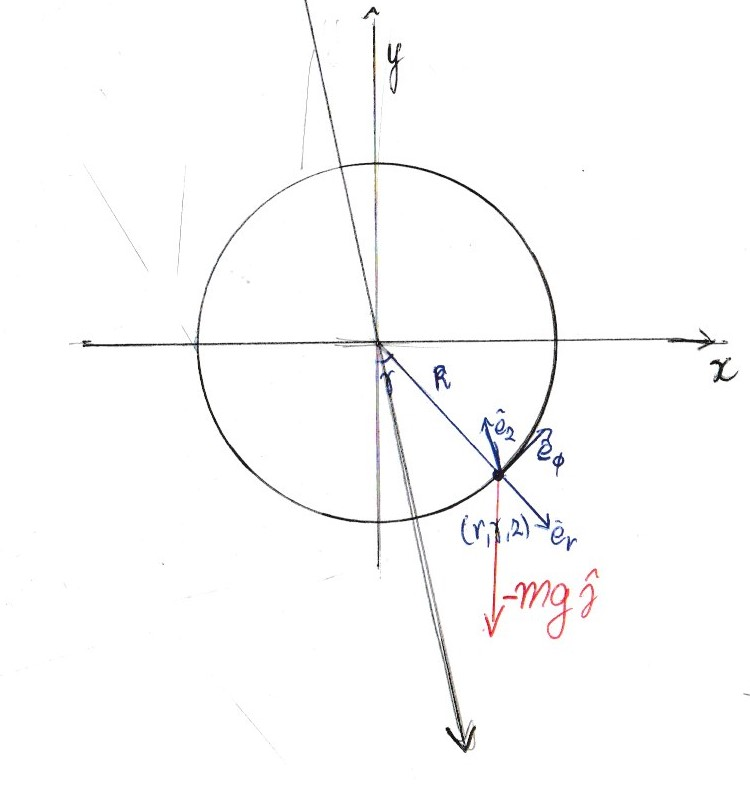
\includegraphics[width=5cm]{coord2.jpg}
	\label{cordinate}
\end{figure} 

As before, we start by writing the applied torque of the system, which will again be exclusively due to gravity on the mass $m$:

\begin{equation*}
	\boldsymbol{\Gamma} = \boldsymbol{r} \times \boldsymbol{F} = R \boldsymbol{e_r} \times mg \boldsymbol{e_y} = mgR\left(\boldsymbol{e_r} \times \left(\cos(\gamma)\boldsymbol{e_r} - \sin(\gamma) \boldsymbol{e_\gamma}\right)\right) = -mgR \sin(\gamma) \boldsymbol{e_z}
\end{equation*}

\begin{equation}
	\label{torque2}
	\boldsymbol{\Gamma} = -mgR \sin(\gamma) \boldsymbol{e_z}
\end{equation}
Wher
Then, we calculate the angular momentum. For this, we will have to consider two sources: One, from the gyroscope, $\boldsymbol{J_1} = I \dot{\gamma} \boldsymbol{e_z}$, and the other from the mass:
$$\boldsymbol{J_2} = \boldsymbol{r} \times \boldsymbol{p} = R \boldsymbol{e_r} \times mR \dot{\gamma} \boldsymbol{e_\gamma} = R^2 \dot{\gamma} \boldsymbol{e_z}$$

Thus, our total angular momentum will be:

\begin{equation}
	\label{angular2}
	\boldsymbol{J} = \boldsymbol{J_1} + \boldsymbol{J_2} = \left(I + mR^2\right) \dot{\gamma} \boldsymbol{e_z} 
\end{equation}

Then, we follow the same procedure that was used in the last section and differentiate \ref{angular2} with respect to time:

\begin{equation}
	\label{djdt}
	\frac{d\boldsymbol{J}}{dt} =\left(I + mR^2\right) \ddot{\gamma} \boldsymbol{e_z}
\end{equation}

Combining equations \eqref{fund}, \eqref{torque2} and \eqref{djdt},  we will get that:

$$\left(I + mR^2\right) \ddot{\gamma} \boldsymbol{e_z} = -mgR \sin(\gamma) \boldsymbol{e_z} $$

If we restrict ourselves only to small $\gamma$ and rearrange, we will get that:

\begin{equation}
	\ddot{\gamma} + \frac{mgR}{I + mR^2} \gamma = 0
\end{equation}

Which is the equation for a simple harmonic oscillator with period $T$:

\begin{equation}
	T = 2\pi\sqrt{\frac{I + mR^2}{mgR}}
\end{equation}

Finally, we can isolate I and get the final expression that we will use to calculate it:

\begin{equation}
	\label{InertiaEq}
	I = mR\left(\frac{g T^2}{4\pi^2} - R\right)
\end{equation}

\section{Experimental Procedure}

\subsection{Methodology}
To attain every objective stated, we must measure three things\footnote{To see this, one must look at equation \eqref{Omegaomega}}:
The distance between the center of mass and the point of contact, $d$ ; the frequency of precession, $\Omega$; and the frequency of rotation, $\omega$.

Thus, we must begin by measuring the distance between the center of mass and point of contact. This is done with the help of indications present in our gyroscope, put there
by the manufacturer, and calipers to get more precise measurements.

Then, we put the gyroscope on its support and start spinning. With the help of a digital counter, we measure the frequency of rotation. 
We therefore start measuring the period of one full precession, which can be trivially transformed into a frequency. After that is done, we again measure the frequency of rotation so we can average them out and get a more accurate measurement.

We then repeat this 5 times with different initial rotation frequencies, and then repeat this process for 4 different values of $d$.
In this manner, we get a sizeable dataset to work with, study the relation between the frequencies and use standard techniques to infer the value of I. 

Then, we turn our gyroscope into a pendulum by placing its axis of symmetric horizontally with the help of a support. We then 
add small masses to it and perturb it slightly. Finally, we measure the period of the oscillation, and repeat this process by adding masses.
With this, we will calculate the moment of inertia as specified in the last part of the theoretical overview.

\subsection{Measurements}
\subsubsection{Gyroscope}
We begin by plotting the data we have acquired for all the different distances that were measured\footnote{It should be noted that a positive precession frequency indicates that it is in the same direction as the rotation, and a negative one indicates that it is opposite to it. This will be further discussed during the Results section.}:


\begin{figure}[h!]
	\label{foda}
	\caption{Frequency of precession as a function of the period of rotation for different values of the distance between the point of contact and the center of mass.}
	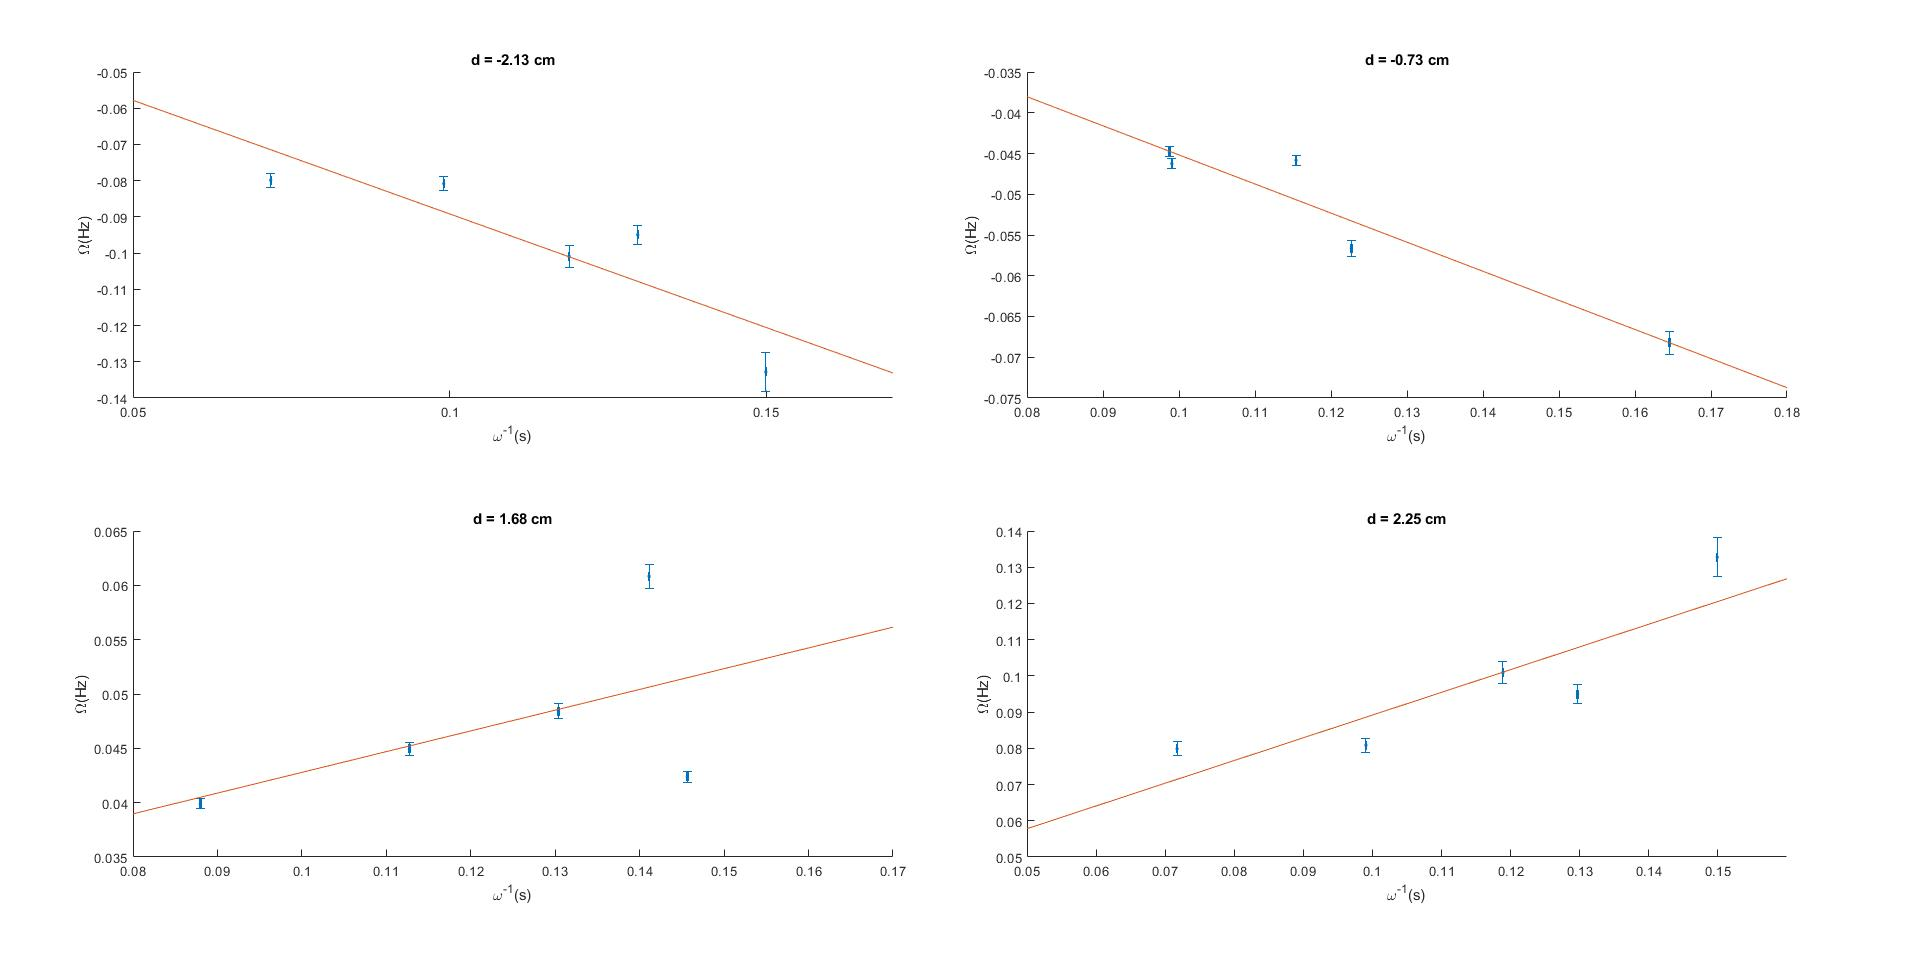
\includegraphics[width=\textwidth]{correct.jpg}
\end{figure} 

Moreover, we represent the coefficients from the linear regressions and their respective uncertainties, since they correspond exactly to the $\omega \Omega$ that we will graph as a function of distance:

\begin{table}[H]
	\centering
  \caption{Values acquired from the linear regression for the different distances.}
  \begin{tabular}{|c|c|}
    \hline
    $d(m)$ & $\Omega \omega (s^{-2})$\\
        \hline
    $(-2.130 \pm 0.005) 10^{-2}$  & $-0.62 \pm 0.22$ \\
    \hline
    $(-0.76 \pm 0.005) 10^{-2}$ & $-0.357 \pm 0.060$ \\
    \hline
    $(1.68 \pm 0.005)10^{-2 }$ & $0.19 \pm 0.13$\\
    \hline
    $(2.25 \pm 0.005)10^{-2}$ & $0.627 \pm 0.17$\\
    \hline
  \end{tabular}
  \label{tabl:Omom}
\end{table}

From equation \eqref{Omegaomega}, we know that if we do a linear regression of $\Omega \omega$ with respect to $d$, our $a$ parameter\footnote{This comes from the linear regression  $\Omega \omega = a d + b$} will give us $\frac{Mg}{I}$, from which we can calculate the moment of inertia, $I$. The results from Table \ref{tabl:Omom} are plotted in Figure \ref{foda2}, where the line of best fit has linear coefficient equal to:

\begin{equation}
  \label{result1}
  a = \frac{Mg}{I} = (26.57 \pm 0.09)10 m^{-1}s^{-2}
\end{equation}

\begin{figure}
	\centering
	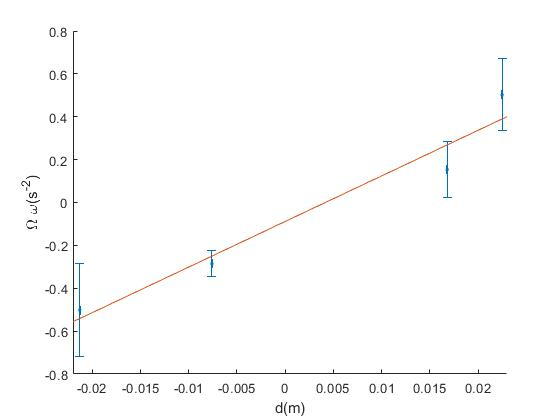
\includegraphics[width=0.5\textwidth]{part2.jpg}
	\caption{Product of the frequencies as a function of the distances between the points of contact and the centers of mass.}
	\label{foda2}
\end{figure} 



Which, since we know both the mass of the gyroscope $M = 3kg$ and the acceleration due to gravity $g = 9.81 m/s^2$, we can rearrange and get an expression for the moment of inertia $I$. Doing that and correctly propagating the data, we get that:

\begin{equation}
  \label{Inertia1}
  I = 1.1 \pm 0.10 m^2kg
\end{equation}

Since we want to get more precise estimate, we will want to get a $95\%$ confidence interval, for which we will need to calculate the the degrees of freedom of $I$, which can be obtained through the Welch-Satterthwaite formula:

$$\nu_{eff} = \frac{u^4(I)}{\frac{c_a u^4(a)}{\nu_a}} =\frac{1}{\frac{1}{\nu_a}} = \nu_a $$


Where $\nu_a = n - 2 = 2$. Trivially, we get that $\nu_{eff} = 2$. Using a standard lookup table for the coverage factor, we get a $95\%$ interval of:
\begin{equation}
\label{inertia2}
I \in [0.67, 1.53]	
\end{equation}
  


\subsubsection{Pendulum}
Just as before, we start by graphing our data and then proceed to calculate the desired coefficients. However, if one inspects Equation \eqref{InertiaEq}, they should realize that if we have $m$ as a function of $\frac{1}{R\left(\frac{g T^2}{4\pi^2} - R\right)}$, the linear coefficient $a$ will coincide with the moment of inertia. This solution, although not very elegant, is what we will be using. Therefore, we have that, for the measured $R = $ that we had  

\begin{figure}[H]
	\caption{Mass as a function of $\frac{1}{R\left(\frac{g T^2}{4\pi^2} - R\right)}$ }
	\centering
	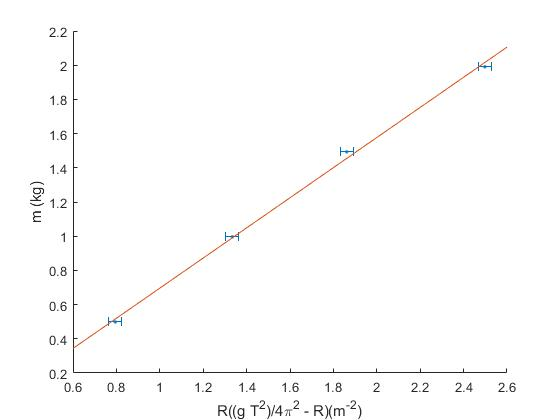
\includegraphics[width=0.5\textwidth]{part3.jpg}
	\label{foda3}
\end{figure} 

And calculating $a$ in the same manner as before, we have that the moment of inertia calculated in this section is:
\begin{equation}
\label{inertia}
	a = I = \left(1.44 \pm 0.23\right) m^2 kg
\end{equation}


\section{Results}

Qualitatively, the gyroscope moved as expected: When we had a negative value for the distance, meaning that the center of mass was below the point of contact, we observed that the direction of precession was opposite to that of rotation; that is, if we rotated the gyroscope clockwise, its precession would happen anticlockwise and vice versa. The opposite happened for positive values of the distance, in which the direction of precession matched that of rotation.

To reflect this in the data, we chose to assign positive values of precession frequency to positive values of the distance, and negative values of it to negative values of the distance. Obviously, none of the theoretical machinery employed would work if this wasn't the case, but it is still worth noting since it might appear strange at first sight to see a negative frequency.

Furthermore, the data reproduced very faithfully what was theoretically expected of it: For a fixed $d$, there was an inversely proportional relationship between the frequency of precession and the frequency of rotation; For varying $d$, there was a directly proportional relationship between it and the product of the frequencies (which should be roughly constant for a given $d$). All in all, the data for this section is, within reasonable bounds, reason for celebration.

As for the moment of inertia, the two results complement each other very nicely. Naively, one might be annoyed by the fact that they are in fact distinct by a reasonable amount, but one must not forget that this isn't merely a theoretical endeavor, but takes place in the real world. This by itself implies that there are statistical uncertainties in measurement, and the whole of uncertainty analysis exists to deal with that.

Therefore, to make use of the tools provided to us, we must realize that the $95\%$ confidence interval calculated in equation \eqref{inertia2} and the interval of standard uncertainty obtained in equation \eqref{inertia} have a very big overlap. This means that both results are in complete agreement with each other. 

\section{Final Discussion}

In this, we have successfully studied the movement of the gyroscope and its many facets, calculating its moment of inertia and reproducing theoretical results to a good amount of precision. As such, every objective proposed in the beginning of the paper has been reached.

The biggest shortcoming was surely related to the way in which frequencies of precession were measured, given that it was done almost entirely by human input. As such, any followup to this experiment should confirm that another way of measuring those periods -- preferably electronically -- is done, as that was the main source of resolutional uncertainty in this experiment. A more detailed study could be done by collecting a larger amount of data, for both more values of $d$ and more diverse initial rotational frequencies. 

\printbibliography
\end{document}
